\subsection{Ay-Matak}
\label{sec:specie-ay-matak}

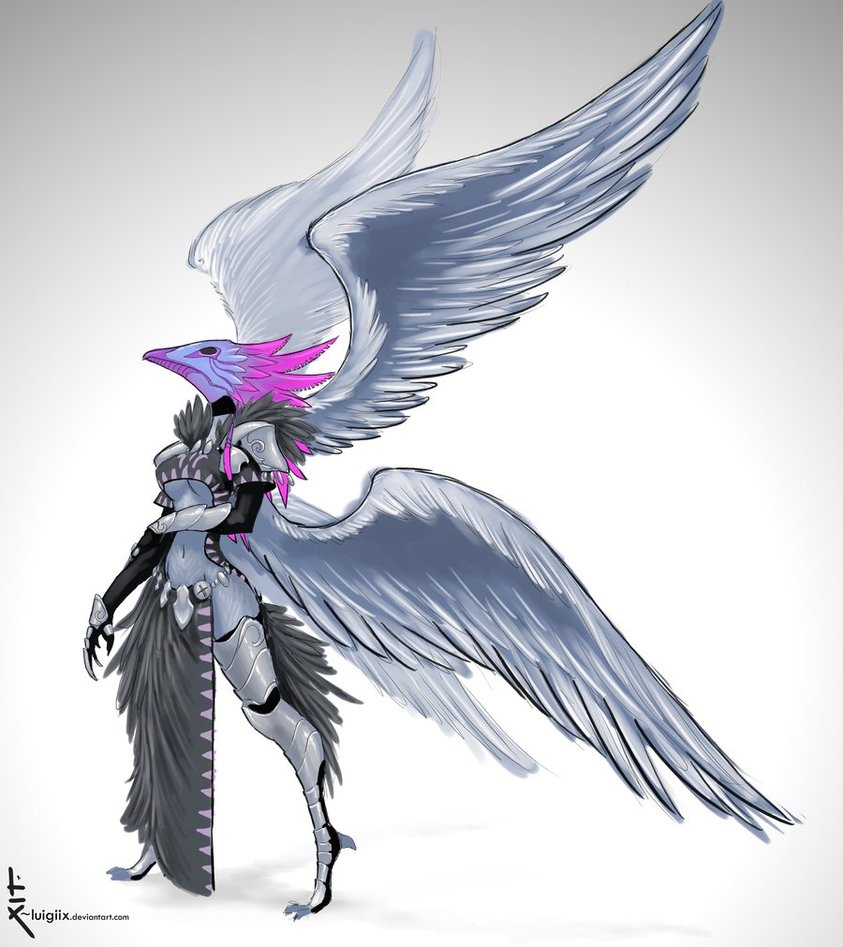
\includegraphics[width=\linewidth]{bird_race_f_concept_by_luigiix-d52w3as}

\begin{redtable}{\linewidth}{@{}L{.35}@{}L{.65}@{}}
  \textbf{Singular} & Matak\\
  \textbf{Plural} & Ay-Matak\\
  \textbf{Adjective} & Matakian\\
  \textbf{Height} & 135-170cm\\
  \textbf{Weight} & 45-65kg\\
  \textbf{Gender Ratio} & 40\% Male / 60\% Female\\
  \textbf{Reproduction} & Oviparity (Eggs)\\
  \textbf{Maturity} & 15 years\\
  \textbf{Lifespan} & 75 years\\
  \textbf{Language} & Kitabian\\
  \textbf{Diet} & Omnivore\\
  \textbf{Homeworld} & Kitaba (Lost)\\
  \textbf{\hyperref[sec:sector-atb]{ATB preference}} & \hyperref[sec:sector-atb]{B-W-H}
\end{redtable}

The Ay-Matak are an avian-like alien species from the world of Kitaba. They were one of the founding races of a Federation that spanned the galaxy before the Surge, renowned for being itinerant wanderers and creative artists. Matakian society focused on culture over conquest, but did not shy away from confrontation when it became unavoidable.

To create a Matak character, please refer to the \textit{\hyperref[sec:rules-creation]{Character creation section}}

\begin{genericsection}{Background}
Kitaba was rumoured to have a tall, dense forest that covered the entire planet and boasted a rich and diverse ecosystem. An overabundance of resources meant that the Ay-Matak had little need to compete with each other. Matakian society evolved to compete culturally rather than physically, leading to a rich and complex history of artistic endeavour. Arts that use an abundance of colour or visual stimuli are especially valued by the Ay-Matak.\\

Matakian governance also revolved around artistic endeavour, with their leaders usually a person of great cultural importance. Democracy was usually limited to recognizing the cultural importance of an individual. Once a Matak achieved that recognition they were able to join the select few who governed and directed Matakian society.
\end{genericsection}

\begin{genericsection}{Physiology}
Ay-Matak are typically shorter and lighter than other bipedal humanoids. They have two pairs of wings that enable them to fly, but they have a pair of functional legs that they use to walk on the ground. Their beak is solid and sharp along the sides, but the tip is made out of softer material so that is flexible enough to produce a variety of sounds.\\

The feathers of a male Matak is always more colourful than the female. Females are usually only limited to whites, greys and blacks.
\end{genericsection}

\begin{genericsection}{Male Names}
Andomion, Antakon, Artenaeon, Demoleo, Dralop, Entardion, Eraton, Eratro, Heliodo, Ikotu, Kalipon, Koron, Lokinu, Melaleimon, Myrodon, Panolio, Taramio, Teladon, Tridru, Tyrorion
\end{genericsection}

\begin{genericsection}{Female Names}
Agara, Alanie, Aldorria, Anakia, Atria, Bellaleta, Belliana, Hallia, Iripira, Karellia, Katia, Kynie, Laleta, Nerian, Nolanta, Obemona, Peneleta, Talitian, Tiakia, Utriema
\end{genericsection}

\begin{genericsection}{Secondary Names}
Ay-Matak do not take family names, but instead earn cultural "\textit{titles}" for their last well-known greatest achievement. For example, \textit{Andomion, painter of 'Matak Lost'}. Those without a great achievement usually go by their occupation, birthplace, spacecraft name, or include the name of their mother ("\textit{hatchling of Anakia}").
\end{genericsection}
